\subsection{带RDMA和SHM的环形缓冲区}
\label{socksdirect:subsec:lockless-queue}

\iffalse
\begin{figure}[t]
	\centering
	
\includegraphics[width=0.4\textwidth]{images/fixme.pdf}
	
	\caption{队列的性能比较。}
	\label{socksdirect:fig:queue-performance}
\end{figure}
\fi

\begin{figure}[t]
	\centering
	\subfloat[传统环形缓冲区。]{
		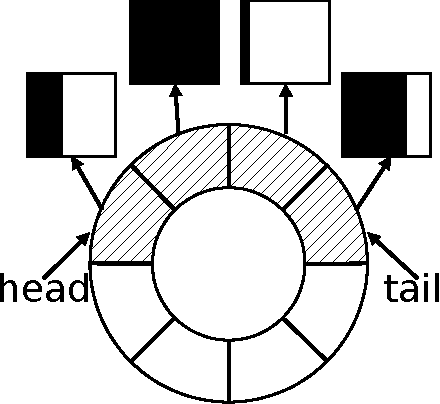
\includegraphics[width=0.3\textwidth]{images/ringbuffer_traditional}
		\label{socksdirect:fig:ringbuffer-traditional}
	}
	\hspace{0.02\textwidth}
	\subfloat[\sys.]{
		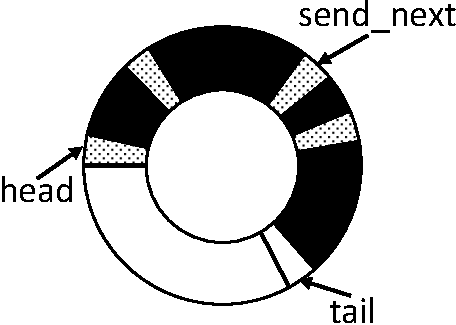
\includegraphics[width=0.32\textwidth]{images/ringbuffer_new}
		\label{socksdirect:fig:ringbuffer-new}
	}
	
	\caption{环缓冲数据结构。 阴影部分是包元数据,黑色部分是有效载荷。}
\end{figure}

传统上,网络堆栈使用环形缓冲区从NIC发送和接收数据包。
如图 \ref {socksdirect:fig:ringbuffer-traditional}所示,它会导致缓冲区管理开销和内部碎片。
传统的NIC支持有限数量的环形缓冲区,因此多个连接可以通过一个环形缓冲区进行复用,这种设计可以将有效负载移动到每个连接缓冲区而无需复制。
幸运的是,RDMA编写动词开辟了新的设计可能性。
我们的创新是拥有\emph {每个套接字连接一个环形缓冲区}并将数据包背靠背存储,如图 \ref {socksdirect:fig:ringbuffer-new}所示。
发送方确定环形缓冲区和偏移量(即\emph {tail}指针),然后使用RDMA写动词将数据包写入远程端内存中的尾指针。
在传输过程中,接收器CPU不需要做任何事情。
当接收器应用程序调用\texttt {recv}时,数据从\emph {head}指针中出列。
SHM的过程类似,因为SHM和RDMA都支持写原语。

要判断环形缓冲区是否已满,发送方将保持\textit {queue credits}计数,指示环形缓冲区中的空闲字节数。
当发件人将数据包入队时,它会消耗信用。 当接收器使消息出列时,它会在本地递增计数器,并在计数器超过环形缓冲区大小的一半时在发送者的内存中写入\textit {credit return flag}。 发送者在检测到标志时重新获得队列信用。
请注意,此机制与拥塞控制无关; 后者由NIC硬件处理 \cite {zhu2015congestion}。

\textbf {发送和接收方的两个环形缓冲区副本。}
上述机制仍然会在发送端引起缓冲区管理,因为发送方需要在缓冲区中构造RDMA消息。
其次,它不支持容器实时迁移,因为RDMA队列中的剩余数据很难迁移。
第三,我们的目标是批量处理小消息以提高吞吐量。
为此,我们在发送方和接收方都保留了环形缓冲区的副本。
发送方写入其本地环形缓冲区,并调用RDMA以使发送方与接收方同步。
我们为每个环形缓冲区使用RDMA RC QP,并维护一个机上RDMA消息的计数器。
如果计数器未超过阈值,则为每个socket \texttt {send}操作发送RDMA消息。
否则,不发送消息,\emph {send\_next}标记第一个未发送的消息。
完成RDMA写入后,我们会在图 \ref {socksdirect:fig:ringbuffer-new}中发送包含所有未发送更改的消息(\emph {send \_next}到\emph {tail})。
这种自适应批处理机制可最大限度地减少空闲链路上的延迟,并最大化繁忙链路上的吞
对于SHM,我们只有一个由两个进程共享的环形缓冲区副本,并且同步由高速缓存一致性硬件完成。

%Before sending, sender clears header of the next message to prevent the receiver from considering junk data in the ring buffer to be a message. Next, sender writes payload, then writes header, finally advances \textit{tail}. Receiver polls \textit{isvalid} at \textit{head} pointer, then copies the message, finally advances \textit{head}.
%For RDMA, the sender maintains a local copy of ring buffer, and we use one-sided RDMA write to synchronize updates from sender to receiver.
%For RDMA, it is known that one-sided verbs has higher throughput than two-sided ones; short messages has lower throughput than large ones~\cite{kalia2014using,kaminsky2016design}.
%In light of this, the inter-host queue has two identical copies in pinned sender and receiver memory, and we use one-sided RDMA write to synchronize updates from sender to receiver.
%\libipc{} polls CQ to limit the number of in-flight (sent but not acknowledged) messages, which is not only required by RDMA NIC, but also enables \emph{adapative batching}~\cite{li2016clicknp,li2017kv}.
%When a message is enqueued to the ring buffer and the RDMA send queue is not full, it is immediately sent as an RDMA message.
%When \libipc{} polls CQ and finds an empty slot in send queue, it sends all queued but unsent data in queue as an RDMA message, because the messages are stored back-to-back in the queue.


\textbf {有效载荷和元数据之间的一致性。}
对于SHM,英特尔和AMD的X86处理器提供了整体商店订购 \cite {sewell2010x86,intel-manual},这意味着其他内核按照与编写时相同的顺序观察到两次写入。一个8字节的\texttt {MOV}指令是原子的,所以写一个标题是原子的。由于发送方在有效负载之后写入标头,因此接收方将读取一致的消息因此,不需要存储器栅栏指令。

因为RDMA不能确保消息中的写入顺序 \cite {infiniband2000infiniband},我们确实需要确保消息完全到达。虽然在使用go-back-0或go-back-N loss recovery~ \cite {dragojevic2014farm}的RDMA网卡中观察到消息写入顺序,但对于具有选择性重传的更高级NIC,情况并非如此 \cite {mprdma,mittal2018revisiting} 。在\libipc {}中,发送方使用\textit {RDMA write with immediate}动词在接收方生成完成。接收器轮询RDMA \emph {完成队列}而不是环形缓冲区。 RDMA确保接收器上的高速缓存一致性,并且在将数据写入\libipc {}环形缓冲区 \cite {infiniband2000infiniband}之后保证完成消息。


\textbf {平摊轮询开销。}
当不经常使用套接字时,轮询环缓冲区会浪费接收器的CPU周期。我们使用两种技术分摊轮询开销。
首先,对于RDMA队列,我们​​利用RDMA NIC将事件通知复用到单个队列中。
每个线程对所有RDMA QP使用\emph {共享完成队列},因此它只需要轮询一个队列而不是所有每个套接字队列。

其次,每个队列可以在\textit {polling}和\textit {interrupt}模式之间切换。监视器的队列始终处于轮询模式。每个队列的接收者维护一个连续空轮询的计数器。当它超过阈值时,接收器向发送器发送消息,通知队列正在进入中断模式,并在短时间后停止轮询。当发送方以中断模式写入队列时,它还会通知监视器,监视器将通知接收方恢复轮询。


%\RED{Need a performance comparison figure of ring buffer architectures. (traditional ring buffer, new ring buffer, intra, inter, x axis: msg size, y axis: throughput)}

\subsection{零拷贝}
\label{socksdirect:subsec:zerocopy}

\begin{figure}[t]
	\centering
	\subfloat[服务器内SHM。 1)获取物理页面并设置写入时复制; 2)通过SHM发送页面地址; 3)映射收到的页面; 4)(可选)在发送者写入/ memcpy / recv时重新映射。]{
		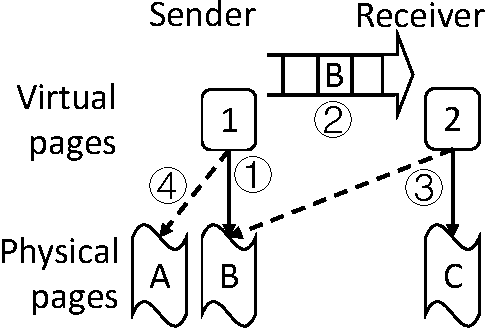
\includegraphics[width=0.44\textwidth]{images/zerocopy_intra}
		\label{socksdirect:fig:zerocopy-intra}
	}
	\hspace{0.02\textwidth}
	\subfloat[服务器间RDMA。 1)获取物理页面并设置写入时复制; 2)从池中获取免费页面; 3)通过RDMA发送数据; 4)通过RDMA发送页面地址; 5)地图收到的页面; 6)将未映射的页面返回到池。]{
		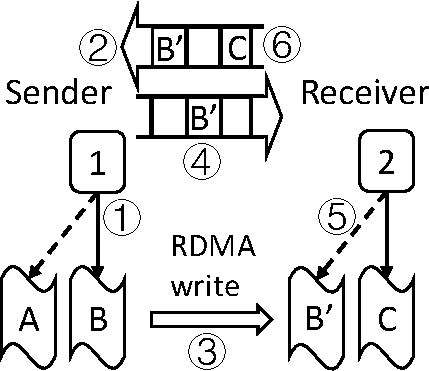
\includegraphics[width=0.42\textwidth]{images/zerocopy_inter}
		\label{socksdirect:fig:zerocopy-inter}
	}
	
	\caption{发送零拷贝页面的过程。}
\end{figure}


正如第 \ref {socksdirect:subsec:per-byte-overhead} 节所讨论的,零拷贝的主要挑战是维护套接字API的语义。
幸运的是,虚拟内存提供了一个间接层,许多作品利用了这种\emph {page remapping}技术。
我们可以将物理页面从发件人的虚拟地址重新映射到接收者,而不是复制。
Linux零复制套接字 \cite {linux-zero-copy}仅支持发送方,通过将数据页设置为写时复制。
但是,许多应用程序经常覆盖发送缓冲区,因此写时复制机制只是将复制从\texttt {send}时间延迟到第一次覆盖时间。
为了实现零拷贝接收,20年前,BSD~ \cite {thadani1995efficient}和Solaris~ \cite {chu1996zero}将应用缓冲区的虚拟页面重新映射到系统缓冲区的物理页面。但是,正如Table~ \ref {socksdirect:tab:operation-performance}所示,在现代CPU上,由于内核交叉和TLB刷新成本,映射一个页面的成本甚至比复制它更高。
最近,许多高性能TCP / IP堆栈 \cite {han2012megapipe,yasukata2016stackmap}和socket-to-RDMA库 \cite {rsockets,socketsdirect}提供标准套接字API和备用零拷贝API,但它们都没有实现标准API的零拷贝。
此外,没有现有的工作支持主机内套接字的零拷贝。



%A sender may write the send buffer after non-blocking \texttt{send}, and the receiver does not know the receive buffer before \texttt{recv}.
% so we can remap virtual address of a buffer to another physical page if the data occupies entire 4~KiB pages.


要启用零拷贝,我们需要修改NIC驱动程序以公开与页面重新映射相关的几个内核函数。
为了分摊页面重新映射成本,我们仅对\texttt {send}或\texttt {recv}使用零拷贝,且有效载荷至少为16~KiB。
而是复制较小的消息。

\textbf {内存对齐。}
页面重新映射仅在发送和接收地址页面对齐且传输包含整个页面时才有效。
我们拦截\texttt {malloc}和\texttt {realloc}函数,并为具有多个4K大小的分配分配4~KiB对齐的地址,因此大多数缓冲区将与页面边界对齐,而不会浪费内存用于小分配。
如果发送消息的大小不是4~KiB的倍数,则最后一块数据将复制到\texttt {send}和\texttt {recv}。

\textbf{讨论非对齐情况:接收之后直接发送,没有读写数据。recv 缓冲区如果不对齐,就默认不做映射,首次访问才 page fault 映射上来;recv 之后直接 send,应用程序不 touch payload 就根本不需要映射到虚拟地址空间。}

%\textbf{Amortize page remapping cost.}


\textbf{减少写时复制。}
当发送者在\texttt {send}之后覆盖缓冲区时,现有设计使用copy-on-write。
复制是必需的,因为发件人可能会读取页面的未写入部分。
由于应用程序几乎总是将缓冲区重用于后续发送操作,因此在大多数情况下会调用copy-on-write,这使得零拷贝在发送方上基本无用。
我们的观察是大多数应用程序不会逐字节写入发送缓冲区。 相反,它们会通过\texttt {recv}或\texttt {memcpy}覆盖发送缓冲区的整个页面,因此无需复制页面的原始数据。
对于\texttt {memcpy},我们调用内核重新映射新页面并禁用copy-on-write,然后执行实际复制。
对于\texttt {recv},旧页面映射将被接收的页面替换。


\textbf {页面分配开销。}
页面重新映射需要内核为每个零拷贝\texttt {send}和\texttt {recv}分配和释放页面。
内核中的页面分配使用全局锁定,这是低效的。 \libipc {}在本地管理每个进程中的可用页面池。
\libipc {}还跟踪收到的零拷贝页面的来源。
当页面未映射时,如果它来自另一个进程,\libipc {}会通过消息将页面返回给所有者。

\textbf {通过SHM安全发送页面地址。}
对于主机内部套接字,我们在用户空间队列中的消息中发送物理页面地址,如图 \ref {socksdirect:fig:zerocopy-intra}中的步骤2所示。
我们必须防止未经请求重新映射任意页面。
为此,\libipc {}调用修改后的NIC驱动程序
获取发送缓冲区的模糊物理页面地址,并通过共享内存队列将地址发送给接收方。
在接收端,\libipc {}调用内核将模糊的物理页面重新映射到应用程序提供的接收缓冲区虚拟地址。

\textbf {RDMA下的零拷贝。}
\libipc {}初始化接收器上的固定页面池,并将页面的物理地址发送给发送者。
发件人管理池。
在发送方上,\libipc {}将发送缓冲区固定,从远程接收器页面池中分配页面以确定RDMA写入的远程地址,如图 \ref {socksdirect:fig:zerocopy-inter}中的步骤2所示。
在接收器上,当调用\texttt {recv}时,\libipc 调用NIC驱动程序将池中的页面映射到应用程序缓冲区虚拟地址。
在重新映射的页面被释放后(例如被另一个\texttt {recv}覆盖),\libipc {}将它们返回给发送方中的池管理器(步骤6)。

%If the OS runs out of memory, \libipc{} unpins pages to reclaim memory.
%For security, kernel validates that page numbers are in the huge-page receive buffer.

%\subsubsection{Zero Copy TCP}
%\label{socksdirect:subsec:zero-copy-tcp}
%
%For TCP connections, we optimize the user-space TCP/IP stack to remove memory copy between \libipc{} and NIC.
%Because the payloads of sent and received packets need to align at 4~KiB page boundary, we leverage scatter-gather support in modern NICs~\cite{mellanox} to separate packet header from application payload.
%%During initialization, \libipc{} queries IP and Ethernet MAC address from the kernel and constructs a packet header template.
%For \texttt{send}, \libipc{} constructs a packet header to a NIC send work request, then fills in the payload buffer address from application. 
%For receiving data, in background, \libipc{} issues NIC receive work requests with a 54-byte buffer to store Ethernet, IPv4 and TCP headers, followed by a page-aligned buffer to store payload.
%%In corner cases where the received header length is not 54 bytes, \libipc{} reassembles the packet.
%Upon \texttt{recv}, the payload buffer is remapped to application.

\subsection{事件通知}
\label{socksdirect:subsec:process-mux}

\textbf {挑战1:在kernel和\libipc {}之间复用事件。}
应用程序轮询来自Linux内核处理的套接字和其他\textit {内核FD}的事件。
轮询内核事件的一种简单方法是每次都调用系统调用(例如\textit {epoll \_wait}),这会产生很高的开销,因为事件轮询几乎是每次发送和接收的频繁操作。
LOS~ \cite {huang2017high}定期用内核FD调用非阻塞\texttt {epoll \_wait}系统调用,这导致延迟和CPU开销之间的权衡。不同的是,
不同的是,\libipc {}创建了一个per-process \textit {epoll thread},它调用\textit {epoll \_wait} syscall来轮询内核事件。每当epoll线程收到内核事件时,应用程序线程将报告该事件以及用户空间套接字事件。

\textbf {挑战2:中断繁忙的进程。}
套接字接管机制(Sec .~ \ref {socksdirect:subsubsec:fork_rdwr})需要一个进程来响应监视器请求。但是,进程可以执行应用程序代码而无需长时间调用\libipc {}。为了解决这个问题,我们设计了一个类似于OS中断的\textit {signal}机制。事件启动器首先轮询接收队列一段时间以进行ACK。如果没有回复,它会向接收器发送Linux \textit {signal}并唤醒进程。

由\libipc {}注册的信号处理程序首先确定进程是执行application还是\libipc {}代码。 \libipc {}在库的入口和出口处设置和清除标志。如果信号处理程序发现进程在\libipc 中,它什么也不做,\libipc {}将在将控制权返回给应用程序之前处理该事件。否则,在将控制权返回给应用程序之前,信号处理程序会立即处理从紧急队列到监视器的消息。
因为\libipc {}被设计为快速且无阻塞,所以消息传递启动器很快就会收到响应。

\textbf {挑战3:让多个线程分时核心。}
对于阻塞操作(例如,阻塞recv,connect和epoll\_wait),\libipc {}首先轮询环形缓冲区一次。如果操作没有完成,而不是无限轮询,\libipc {}调用\textit {sched \_yield}以产生同一核心上的其他进程。如章节 \ref {socksdirect:subsec:bottleneck}中所述,协同多任务处理中的上下文切换仅需要0.4~$\mu$s。但是,应用程序可能需要等待很长时间才能进行外部事件,从而导致频繁的唤醒浪费。在这方面,我们计算连续唤醒,它不处理任何消息,并在达到阈值时将进程置于休眠状态。
如果\libipc {}继续产生一定数量的轮次,它将使自己进入睡眠状态。在睡眠之前,它会向监视器和所有对等方发送消息,以便稍后通过消息将其唤醒。

%\textbf{Handling events from kernel.}
%An application often needs to poll kernel FDs (\textit{e.g.} files and semaphores) together with socket FDs.
%\libipc{} creates a per-process \textit{epoll thread} to poll kernel FDs for all application threads. When it receives a kernel event, it broadcasts the event to application threads via shared memory queues.%\texttt{Epoll\_wait} in \libipc{} will return such kernel events in addition to socket events. Note that Linux allows an event to be received by multiple threads sharing the FD.

%\textbf{Exit.}
%When a process exits, the \texttt{atexit} handler of \libipc{} notifies the monitor and all peers to close connections and mark the queues as dead. However, a process may crash or get killed. In this case, monitor detects process death via \texttt{SIGHUP} of the bootstrap socket (Sec.~\ref{socksdirect:subsubsec:fork_fork}) and notify its peers. When a process switches to \texttt{daemon} mode or \texttt{execve} another program, it first follows the process exit procedure, then calls the system call. After that, \libipc{} is re-initialized.


\subsection{连接管理}
\label{socksdirect:subsec:connection-management}

%Before designing the connection management protocol, we keep the following requirements in mind:
%1) The applications and \libipc{} are not trusted because they are in the same memory address space. We must enforce access control policies outside \libipc{} to prevent access to restricted resources.
%2) Each address and port may be listened by multiple processes, which needs load balancing while avoid starvation.
%3) The applications may be in an overlay network and thus needs address translation. 
%%4) Multiple concurrent connections may be created between two hosts and therefore should be accelerated.
%4) A client should be able to connect to \sys{} and regular TCP/IP hosts transparently, and a server should accept connections from all hosts.

%These design requirements lead to a \emph{monitor} service running as a daemon process in each host.
%Rather than delegating all operations to the monitor, we only delegate connection creation, which forms the control plane.
%From the application's perspective, connection creation is similar to TCP handshake.
%Monitor(s) on the path between client and server applications proxy the handshake commands and help them establish a peer-to-peer queue via shared memory or RDMA.
%If the remote peer does not support \sys{}, all future operations with it will be delegated to the local monitor.
%The detailed procedure is as follows.


\begin{figure}[t!]
	\centering
	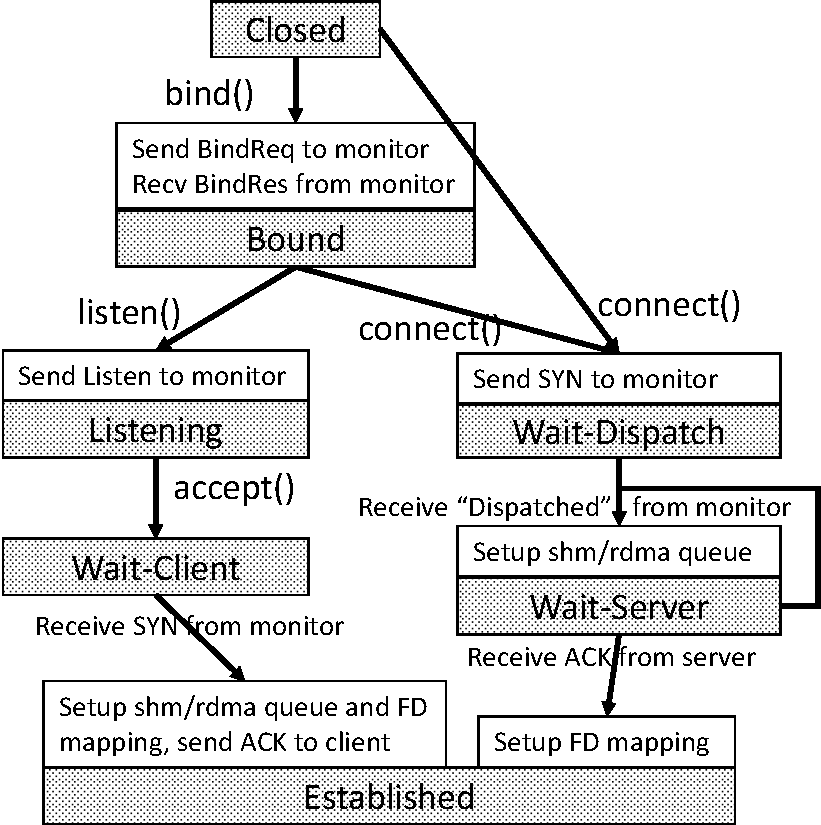
\includegraphics[width=0.6\textwidth]{images/conn-setup-new}
	
	\caption{State machine of connection setup in \libipc{}.}
	\label{socksdirect:fig:conn-setup}
\end{figure}


\subsubsection{FD 重映射表}
\label{socksdirect:subsubsec:fd-remapping-table}



套接字FD和其他FD(例如磁盘文件)共享命名空间,Linux总是分配最低可用FD。
为了保留这种语义而不在内核中分配虚拟FD,\libipc {}拦截所有与FD相关的Linux API并维护\emph {FD重映射表}以将每个应用FD映射到用户空间套接字对象或内核FD。
当FD关闭时,\libipc {}将其放入\emph {FD回收池}。
在FD分配时,\libipc {}首先尝试从池中获取FD。
如果池为空,则通过递增\emph {FD分配计数器}来分配新的FD。
FD回收池和分配计数器在进程中的所有线程之间共享。

\subsubsection{连接建立}


图 \ref {socksdirect:fig:conn-setup}显示了连接建立过程。

\textbf{绑定。}
创建套接字后,应用程序调用\texttt {bind}来分配地址和端口。
由于地址和端口是具有权限保护的全局资源,因此分配由监视器协调。
如图 \ref {socksdirect:fig:conn-setup}所示,\libipc {}将请求发送到监视器。
为了隐藏联系监视器的延迟,如果绑定请求不会失败,\libipc {}会立即返回应用程序,例如,当没有为客户端套接字指定端口时。

\textbf{监听。}
当服务器应用程序准备好接受来自客户端的连接时,它会调用\texttt {listen}并通知监视器。
监视器维护每个地址和端口上的侦听进程列表,以分派新连接。


\textbf{连接。}
客户端应用程序调用\texttt {connect}并发送SYN命令以通过SHM队列进行监视。
现在,监视器需要将新连接分派给侦听应用程序。
在Linux中,新的连接请求在内核的\emph {backlog}中排队。
每次服务器应用程序调用\texttt {accept}时,它都会访问内核以从积压中出列,这需要同步并增加延迟。
相反,我们为每个侦听套接字的线程维护一个每个监听器的积压。
监视器以循环方式将SYN分发给侦听器线程。

当侦听器不接受新连接时,调度与侦听器的连接可能会导致饥饿。
我们设计了一种\emph {work stealing}方法。
当监听器在积压为空时调用\texttt {accept}时,它会请求监视器窃取其他人的积压。
为了避免侦听器和监视器之间的争用,监视器向侦听器发送请求以从积压中窃取。

\textbf {建立点对点队列。}
客户端和服务器应用程序第一次通信时,服务器监视器可帮助它们建立直接连接。
对于主机内部,监视器分配SHM队列并将SHM密钥发送到客户端和服务器应用程序。
对于主机间,客户端和服务器监视器建立新的RDMA QP,并将本地和远程密钥发送到相应的应用程序。
为了减少延迟,当SYN命令分发到监听器的待办事项时,监视器会建立对等队列。
但是,如果SYN被另一个侦听器窃取,则需要在客户端和新侦听器之间建立新队列,如图 \ref {socksdirect:fig:conn-setup}中的Wait-Server状态所示。

\textbf {连接建立的最后步骤。}
服务器设置对等队列后,如图 \ref {socksdirect:fig:conn-setup}左侧所示,服务器应用程序向客户端发送ACK。 ACK包含SYN请求中的客户端FD及其分配的服务器FD。
与TCP握手类似,服务器应用程序可以在发送ACK后将数据发送到队列。
当客户端收到ACK时,如图 \ref {socksdirect:fig:conn-setup}右侧所示,它设置FD映射并可以开始发送数据。


\subsubsection{与常规 TCP/IP 对端的兼容性}


为了与不支持\sys {}和RDMA的对等端兼容,我们需要检测\sys {}功能并回退到TCP / IP。
但是,Linux不支持向TCP SYN和ACK数据包添加特殊选项。
由于中间盒和网络重新排序,使用另一个端口(例如LibVMA~ \cite {libvma})也是不可靠的。
为此,我们首先使用内核原始套接字直接发送带有特殊选项的SYN和ACK数据包,如果不存在特殊选项,则回退到内核TCP / IP套接字。

在客户端,监视器通过网络发送带有特殊选项的TCP SYN数据包。
如果对等体具有\sys {}能力,则其监视器将接收特殊SYN并且知道客户端具有\sys {}能力。
然后,服务器使用特殊选项响应SYN + ACK,包括设置RDMA连接的凭据,以便两个监视器之后可以通过RDMA进行通信。
如果客户端或服务器监视器发现对等方是常规TCP / IP主机,它将使用TCP连接修复 \cite {tcp-connection-repair}在内核中创建已建立的TCP连接。
然后监视器通过Unix域套接字将内核FD发送到应用程序,\libipc {}可以使用内核FD进行未来的套接字操作。


一个棘手的问题是接收的数据包被传递到原始套接字和内核网络堆栈,并且内核将使用RST响应,因为这样的连接不存在。
为避免此行为,监视器会安装\emph {iptables}规则来过滤此类出站RST数据包。

%\begin{figure}[t!]
%	\centering
%	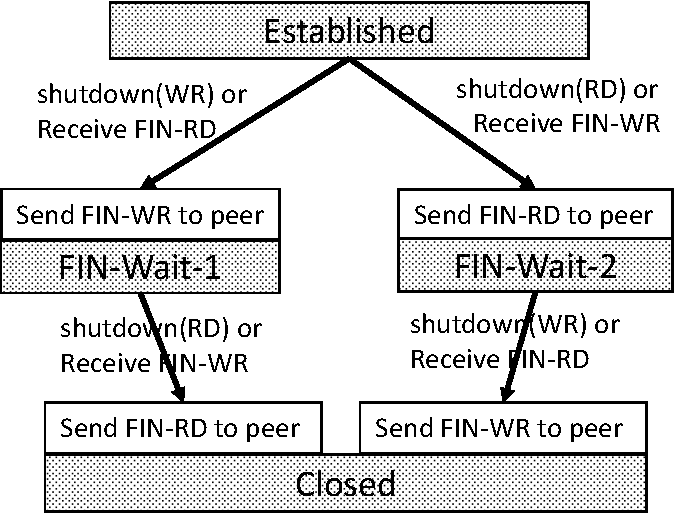
\includegraphics[width=0.25\textwidth]{images/conn-close-new}
%	
%	\caption{State machine of connection close in \libipc{}.}
%	\label{socksdirect:fig:conn-close}
%\end{figure}


\subsubsection{连接关闭}



当应用程序调用\texttt {close}时,\libipc {}会从重映射表中删除FD。
然而,套接字数据可能仍然有用,因为FD可以与其他进程共享,并且缓冲区中可能存在未发送的数据。
我们跟踪每个套接字的引用计数,它在fork上递增,在close时递减。
为了推出未发送的数据,我们需要在对等体之间进行握手,类似于TCP close。
因为套接字是双向的,所以\texttt {close}在发送和接收方向上相当于\texttt {shutdown}。
当应用程序关闭连接的一个方向时,它会向对等方发送\emph {shutdown message}。
对等体以关闭消息响应。
当\libipc {}在两个方向上收到关闭消息时,将删除套接字。


\iffalse

\textbf{\texttt{Bind} and \texttt{listen}.}
A \emph{server} process \texttt{bind}s a socket and needs to detect IP and port conflict. In this case, \texttt{bind} is non-partitionable and goes to the monitor. The monitor also listens on the IP and port in a user-space TCP/IP stack (\textit{e.g.} mTCP~\cite{jeong2014mtcp}, LibVMA~\cite{libvma} or Seastar~\cite{seastar}) to receive connections from other hosts.

A \emph{client} process typically \texttt{bind}s without specifying IP and port, so we need to allocate a unique IP and port for it. For scalability, we partition the loopback IP address space (127.0.0.0/8) and each process allocates IP and port in its range.

\textbf{\texttt{Connect} and \texttt{accept}.}
When a client process connects to a server process on the same host, it sends a \textit{connect request} to the monitor via shared memory queue. When the server process is on another host, it creates a \textit{bootstrap TCP socket} with a special option via the user-space TCP/IP stack. If the server host supports the option, it is a \sys host and its monitor establishes an RDMA connection to the client to speedup later communications. Otherwise, the client process keeps using the bootstrap TCP socket for compatibility.

On a server host, the monitor distributes connect requests to server processes in a round-robin order, and a \textit{backlog} is maintained in each process. If the client is TCP only, the monitor proxies messages between the server process and the user-space TCP/IP stack. If the client is intra-server or RDMA capable, and it is the first time for the client and server processes to communicate, the monitor creates an inter-process queue for the process pair and sends the credentials to both processes via bootstrap sockets. After a server process \texttt{accept}s a connection in the backlog, it sends a message to the client via inter-process queue to create an FD mapping, then the socket is ready for data transmission. As Figure~\ref{socksdirect:fig:conn-setup} shows, connection creation takes three inter-process delays.

Distributing connection to listeners may lead to starvation when a listener does not \texttt{accept} new connections. We devise a \textit{work stealing} approach. When a listener \texttt{accept}s from empty backlog, it requests the monitor to steal from others' backlog. To avoid polling empty backlogs, each listener notifies the monitor when its backlog becomes empty. To avoid contention between a listener and monitor, the monitor sends a request to the listener rather than stealing from the backlog directly.

%\subsubsection{Connection Close}

\textbf{\texttt{Close} and \texttt{shutdown}.}
Connection close is a peer-to-peer operation because only the peer process needs to be notified. If FD is deleted immediately after \texttt{close}, a new connection may reuse the FD while the peer process might not yet have received the close event thus sends data to the wrong connection. To avoid this, we require a handshake between peers.
Because socket is bidirectional, \texttt{close} is equivalent to \texttt{shutdown} on both send and receive directions.
When application shuts down one direction of a connection, it sends a \textit{shutdown message} to the peer. The peer responds with a shutdown message. A process deletes an FD when it receives shutdown messages in both directions.

%In order to achieve high scalability, we separate scalable operations to different processes. To avoid the overhead of contention, \libipc enable the file descriptor allocation by individual process and when a connection is setup, the other peer of the connection gets notified of the file descriptor number by message passing. Since we treat different threads in one process as different processes, we allocate file descriptor of different ranges to each of them to avoid collision. Since file descriptor is managed separately by each process, it is possible that a file descriptor is reused after the connection is closed. Our solution is that resources of a file descriptor is not released until an ACK is received for the close operation.

%Generally, each process in our design is treated as an endpoint in the network. Figure \ref{socksdirect:fig:conn-setup-close} shows the process of connection setup and close. When \textit{socket} is called, the process itself allocate per fd resources. When \textit{listen} is called, monitor is notified of port occupation. During the \textit{connect} operation, monitor first chooses one of the processes listen on this port then coordinates the creation of the shared memory between the two processes and notifies each other of the new connection. When \textit{close} happens, both of the endpoint notify each other and monitor is responsible to destroy the shared memory between them. 

\fi
